\section{CHSH Game}
The CHSH game, also demonstrating the violation of Bell inequality, has the following set up. \\
We have $3$ people, Alice, Bob and the referee. The referee will distribute $x, y$ to Alice and Bob respectively such that $x, y$ are drawn uniformly at random from the set $\{0, 1\}$. Without discussing, Alice and Bob must give $a, b \in \{0, 1\}$ to the referee respectively in their own choices. Alice and Bob wins if
$$a \oplus b = x \land y$$
One na\"ive strategy that Alice and Bob can use is always choosing $a = b = 0$, this way they have a $\frac{3}{4}$ chance of winning the game. \\
If we think about it more generally, and discuss a deterministic strategy, that is:
\begin{align*}
    a: \{0, 1\} &\to \{0, 1\} \\
    x &\mapsto 0 \text{ or } 1 \\
    b: \binset &\to \binset \\
    y &\mapsto 0 \text{ or } 1
\end{align*}
We can demonstrate that for all possible pairs of $(x, y)$, it is impossible to satisfy $a(x) \oplus b(y) = x \land y$ at the same time. There is at most a $\frac{3}{4}$ chance of winning the game. \\
What if we employ a randomized strategy? Before Alice and Bob go into the game, they sample some random variable $\lambda \in \R$ with probability density $p_\lambda$, and choose a deterministic strategy $a_\lambda$ and $b_\lambda$. If we draw out each $\lambda_i$ for all $i \in \{1, \dots, n\}$, each path is a deterministic strategy with winning probability at most $\frac{3}{4}$. Thus, the probability of winning the game using randomized strategy:
$$\Prob{\text{winning}} \le \Sumi{i} p_{\lambda_i} \times 0.75 = 0.75$$
Thus, any \impt{randomized strategy} with \impt{no communication} wins with a probability at most $0.75$; any \impt{hidden variable} theory that is also \impt{local} wins with a probability at most $0.75$.

\subsection{Quantum Strategy - 量子策略}
\begin{theorem}
    By employing a quantum strategy, Alice and Bob can win the game with probability $\cos^2(\frac{\pi}{8})$.
\end{theorem}
\begin{definition}
    A $2$-qubit state $\ketpsi$ is \uimpt{entangled} if $\ketpsi$ cannot be written as $\ket{\psi_1} \otimes \ket{\psi_2}$ where $\ket{\psi_i}$ are $1$-qubit states.
\end{definition}
The quantum strategy is described by a quantum circuit:
\begin{center}
    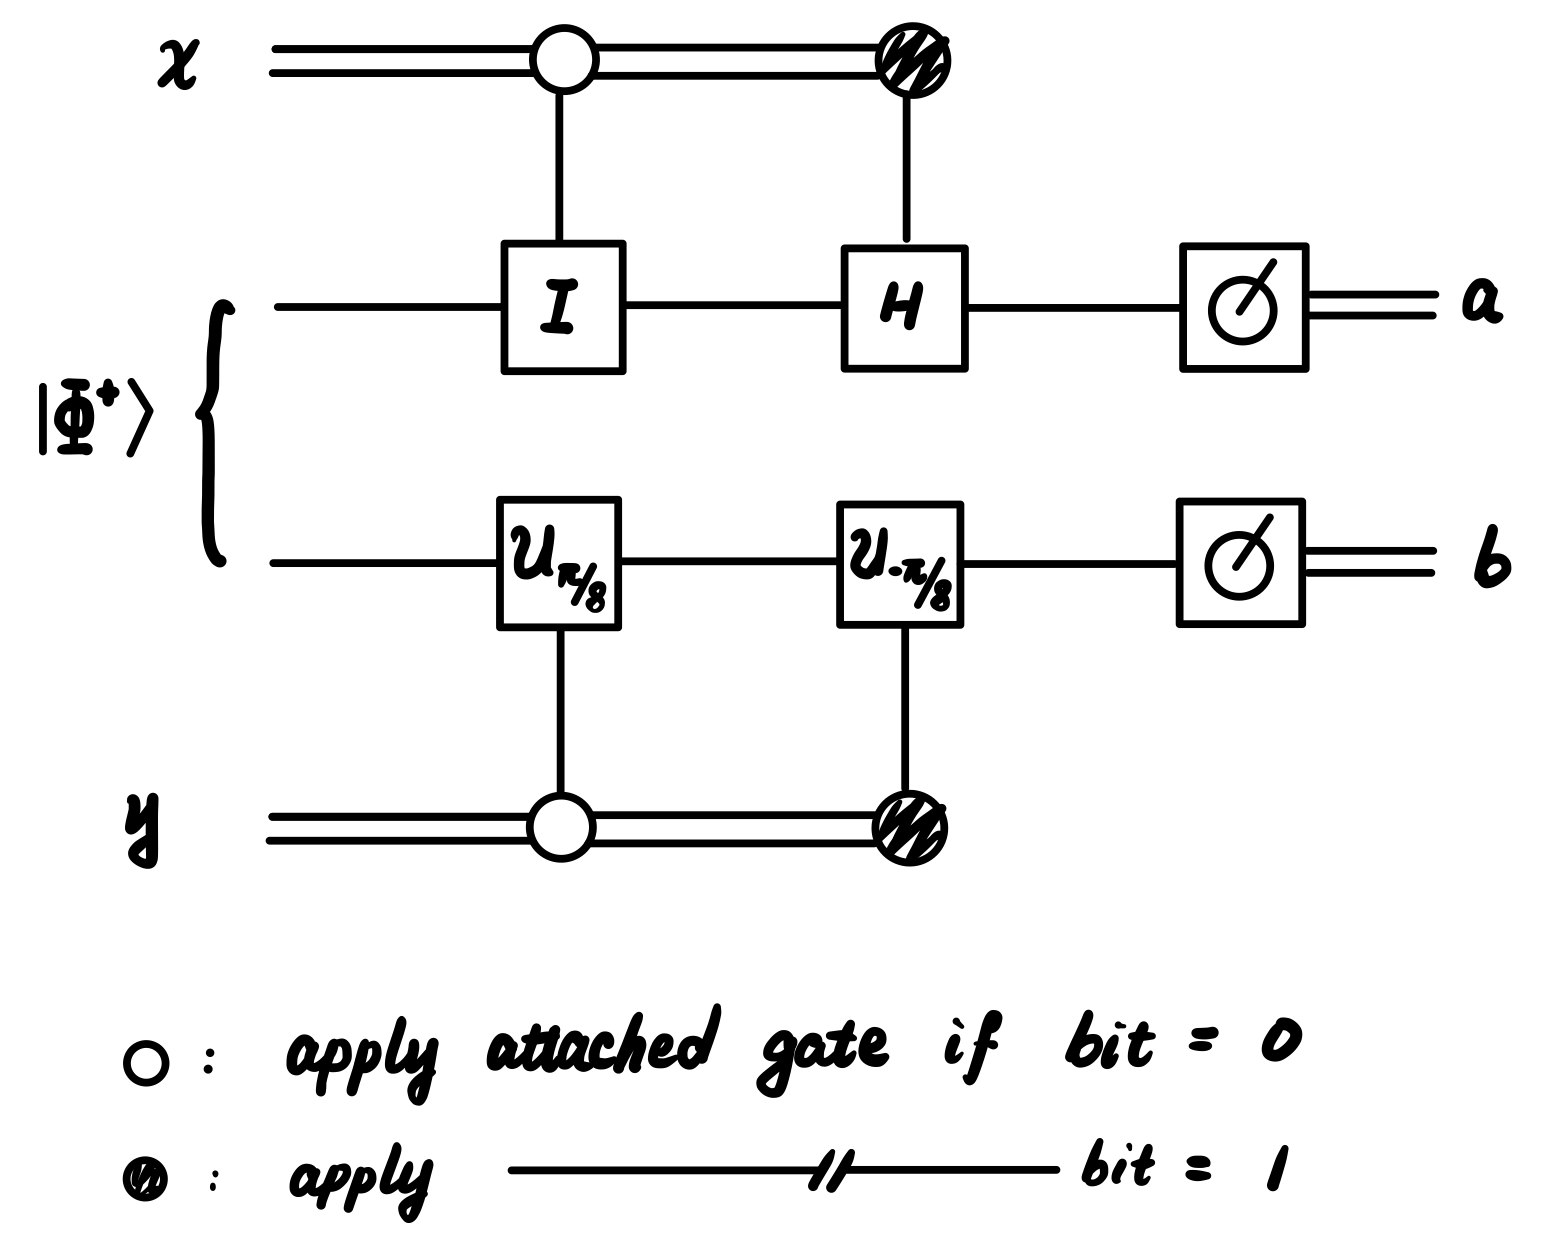
\includegraphics[scale=0.2]{4/chsh.png}
\end{center}
where $\opuni_\theta$ is the following (it can be interpreted as a rotation matrix by angle $\theta$ \impt{clockwise}):
$$\opuni_\theta = \begin{pmatrix}
    \cos \theta & \sin \theta \\
    -\sin \theta & \cos \theta
\end{pmatrix}$$
and $\ket{\Phi^+}$ is also called the EPR pair specified to be:
$$\ket{\Phi^+} = \frac{1}{\sqrt{2}}(\ket{00} + \ket{11})$$
We provide one example case to demonstrate the above probability, where $x = 1$ and $y = 0$:
\begin{align*}
    \ket{\Phi^+} &\to (H \otimes \opuni_{\frac{\pi}{8}}) \\
    &= \id(H \otimes \opuni_{\frac{\pi}{8}})\ket{\Phi^+} \\
    &= \Sumi{\mathbf{x}} \dyad{\mathbf{x}} H \otimes \opuni_{\frac{\pi}{8}} \ket{\Phi^+} \\
    &= \Sumi{\mathbf{x}} \mel{\mathbf{x}}{H \otimes \opuni_{\frac{\pi}{8}}}{\Phi^+}\ket{\mathbf{x}}
\end{align*}
Since $x \land y = 0$, we want $a \oplus b = 0$, meaning that either $a = b = 0$ or $a = b = 1$, that is, we only care about the coefficients for $\mathbf{x} = 00, 11$, which is:
$$\Prob{\mathbf{x} = 00, \mathbf{x} = 11} = \abs{\mel{00}{H \otimes \opuni_{\frac{\pi}{8}}}{\Phi^+}}^2 + \abs{\mel{11}{H \otimes \opuni_{\frac{\pi}{8}}}{\Phi^+}}^2$$
If we expand the first part we have:
\begin{align*}
    \mel{00}{H \otimes \opuni_{\frac{\pi}{8}}}{\Phi^+} &= \frac{1}{\sqrt{2}} \bra{00} (H \otimes \opuni_{\frac{\pi}{8}} \ket{00} + H \otimes \opuni_{\frac{\pi}{8}} \ket{11}) \\
    &= \frac{1}{\sqrt{2}} \bra{00} ((\frac{1}{\sqrt{2}}(\ket{0} + \ket{1}))(\cos\theta\ket{0} - \sin\theta\ket{1}) \\
    &+ (\frac{1}{\sqrt{2}}(\ket{0} - \ket{1}))(\sin\theta\ket{0} + \cos\theta\ket{1})) \\
    &= \frac{1}{2} (\cos\theta + \sin\theta)
\end{align*}
If we do the same thing for $\mel{11}{H \otimes \opuni_{\frac{\pi}{8}}}{\Phi^+}$, we would obtain $\frac{1}{2}(-\sin\theta - \cos\theta)$.
We take the square of each value, add them together, and substitute $\theta = \frac{\pi}{8}$, we get the probability of $\cos^2(\frac{\pi}{8})$.

\subsection{Partial Measurement - 部分测量}
\begin{definition}
    Let $m \le n$ be positive integers. A \uimpt{partial measurement} of the first $m$ qubits of an $n$-qubit state $\ketpsi = \Sumi{\mathbf{x}}\alpha_{\mathbf{x}} \ket{\mathbf{x}}$ is a process that: \\
    1. returns $\mathbf{y} \in \binset^m$ with probability
    $$p_{\mathbf{y}} := \norm{(\bra{\mathbf{y}} \otimes \id^{n - m})\ketpsi}^2 = \Sumi{\mathbf{x}[1:m] = \mathbf{y}} \abs{\alpha_{\mathbf{x}}}^2$$
    2. given $\mathbf{y}$ is returned, the state of the remaining $n - m$ qubits become
    $$\ket{\psi_\mathbf{y}} := \frac{\mel{\mathbf{y}}{\id^{n-m}}{\ketpsi}}{\sqrt{p_{\mathbf{y}}}}$$
\end{definition}
An example of this is given $\ketpsi = \sqrt{\frac{1}{2}} \ket{00} + \sqrt{\frac{1}{4}} \ket{01} + \sqrt{\frac{1}{6}} \ket{10} + \sqrt{\frac{1}{12}} \ket{11}$, if we measure the $1^{st}$ qubit, the probability of getting $0$ is $\frac{3}{4}$ and getting $1$ to be $\frac{1}{4}$, which both coincidentally have the same leftover state after partial measurement to be:
$$\sqrt{\frac{2}{3}}\ket{0} + \sqrt{\frac{1}{3}}\ket{1}$$
\begin{theorem}
    Let $\ketphi$ bet any $n$-qubit state, consider $2$ experiments:
    1. directly measure the first $m$ qubits, obtaining outcome $b$ and post-measurement state $\ket{\phi_b}$. \\
    2. first apply some $(n-m)$-qubit unitary $\opuni$ on the last $n-m$ qubits of $\ketphi$, then measure the first $m$ qubits of $\ketphi$, obtaining outcome $c$ and post-measurement state $\ket{\phi_c'}$. \\
    Then, the distribution of $b, c$ are identical, and $\ket{\phi_c'} = \opuni \ket{\phi_c}$ for all $c \in \binset^m$.
\end{theorem}

\subsection{Alternative Analysis}
Given the partial measurement definition, we can re-analyze the CHSH game. \\
From linear algebra, for two real vectors $\ket{u}$ and $\ket{v}$ of the same dimension, we have:
$$\braket{u}{v} = \norm{\ket{u}} \cdot \norm{\ket{v}} \cdot \cos \theta$$
and if they are quantum states, we further have $\abs{\braket{u}{v}}^2 = \cos^2\theta$. \\
We can consider that Alice measuring first, which is a partial measurement on the first qubit, and get $a$.
For each case of $(x, y)$, we can then consider the probability of Bob measuring the corresponding $b$ so that they can win to be plotted on a 2D Cartesian plane. \\
An example of this is when $(x, y) = (0, 0)$, Alice has $\frac{1}{2}$ of getting $0$ and $1$ respectively. And we want to find the probability of Bob measuring $0$ and $1$ respectively as well, then we have:
\begin{center}
    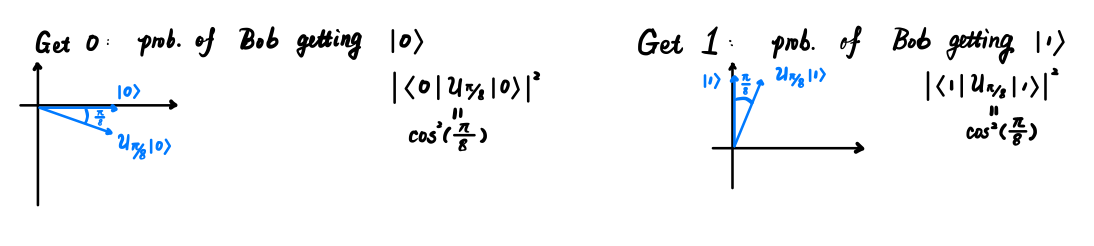
\includegraphics[scale = 0.4]{4/chsh_alt.png}
\end{center}
This process can be applied to each $(x, y)$.

\newpage